\subsection{The logarithmic function}

In his paper \cite{shannon1948mathematical}, Claude Shannon addresses the fundamental problem of communication, which technically consists of reproducing a message selected at one point from another point. He stresses that the semantic aspects of communication, such as the meaning of messages, are unimportant. What matters is that the actual message comes from a set of possible messages, and the system must be designed to work for every possible selection.

To quantify the information produced when a message is selected from a set, Shannon proposed a measure based on the logarithm. This measure is practical for several reasons. Firstly, it is more practically useful, as it allows important engineering parameters such as time, bandwidth and number of relays to be expressed linearly. Secondly, it better matches our intuition as to the appropriate measurement, as it allows linear comparisons with common standards. Finally, it is mathematically more suitable, as many limit operations are simple in logarithmic terms but would require awkward reformulation in terms of the number of possibilities.

The choice of logarithmic base corresponds to the choice of a unit for measuring information. The use of base 2 leads to units called "bits", while base 10 leads to units called "decimal digits". In certain analytical contexts, base "e" may also be used, giving rise to units called "natural units". Switching from one base to another simply requires multiplication by the logarithm of the ratio between the bases.In the context of Wordle, the words are a sequence of letters that can be converted to bits so we will use the base 2.

An alternative to the logarithm would be the square root. In some cases, this function could be used to give less weight to extreme values.



\begin{figure}[!ht]
\centering
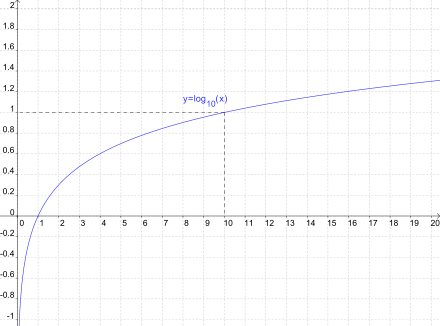
\includegraphics[scale=0.7]{images/logarithme.png}
\caption{logarithm curve \cite{wiki_log}}
\label{logarithm}
\end{figure}

\newpage
